%%%%%%%%%%%%%%%%%%%%%%%%%%%%%%%%%%%%%%%%%%%%%%%%%%%%%%%%%%%%%%%%%%%%%
%% This is a (brief) model paper using the achemso class
%% The document class accepts keyval options, which should include
%% the target journal and optionally the macuscript tye
%%%%%%%%%%%%%%%%%%%%%%%%%%%%%%%%%%%%%%%%%%%%%%%%%%%%%%%%%%%%%%%%%%%%%
\documentclass[journal=jacsat,manuscript=article]{achemso}

%%%%%%%%%%%%%%%%%%%%%%%%%%%%%%%%%%%%%%%%%%%%%%%%%%%%%%%%%%%%%%%%%%%%%
%% Place any additional packages needed here.  Only include packages
%% which are essential, to avoid problems later.
%%%%%%%%%%%%%%%%%%%%%%%%%%%%%%%%%%%%%%%%%%%%%%%%%%%%%%%%%%%%%%%%%%%%%
\usepackage[version=3]{mhchem} % Formula subscripts using \ce{}
\usepackage{graphicx}

%%%%%%%%%%%%%%%%%%%%%%%%%%%%%%%%%%%%%%%%%%%%%%%%%%%%%%%%%%%%%%%%%%%%%
%% If issues arise when submitting your manuscript, you may want to
%% un-comment the next line.  This provides information on the
%% version of every file you have used.
%%%%%%%%%%%%%%%%%%%%%%%%%%%%%%%%%%%%%%%%%%%%%%%%%%%%%%%%%%%%%%%%%%%%%
%%\listfiles

%%%%%%%%%%%%%%%%%%%%%%%%%%%%%%%%%%%%%%%%%%%%%%%%%%%%%%%%%%%%%%%%%%%%%
%% Place any additional macros here.  Please use \newcommand* where
%% possible, and avoid layout changing macros (which are not used
%% when typesetting).
%%%%%%%%%%%%%%%%%%%%%%%%%%%%%%%%%%%%%%%%%%%%%%%%%%%%%%%%%%%%%%%%%%%%%
\newcommand*{\mycommand}[1]{\texttt{\emph{#1}}}

%%%%%%%%%%%%%%%%%%%%%%%%%%%%%%%%%%%%%%%%%%%%%%%%%%%%%%%%%%%%%%%%%%%%%
%% Meta-data block
%% ---------------
%% Each author should be given as a separate \author command.
%%
%% Corresponding authors should have an e-mail given after the author
%% name as an \email command.
%%
%% The affiliation of authors is given after the authors; each
%% \affiliation command applies to all preceding authors not already
%% assigned an affiliation.
%%
%% The affiliation takes an option argument for the short name.  This
%% will typically be something like "University of Somewhere".
%%
%% The \altaffiliation macro should be used for new address, etc.
%%%%%%%%%%%%%%%%%%%%%%%%%%%%%%%%%%%%%%%%%%%%%%%%%%%%%%%%%%%%%%%%%%%%%
\author{Robert Jensen}
\author{Thomas Andersen}
\author{Anders Nierhoff}
\affiliation{CINF, Department of Physics, Technical University of Denmark, Fysikvej, Building 312, 2800 Kgs. Lyngby, Denmark.}
\author{Thomas Pedersen}
\author{Ole Hansen}
\affiliation{CINF, Department of Micro- and Nanotechnology, Technical University of Denmark, \O rsteds Plads, Building 345B, 2800 Kgs. Lyngby, Denmark.}
\author{S\o ren Dahl}
\author{Ib Chorkendorff}
\email{ibchork@fysik.dtu.dk}
\affiliation{CINF, Department of Physics, Technical University of Denmark, Fysikvej, Building 312, 2800 Kgs. Lyngby, Denmark.}

%%%%%%%%%%%%%%%%%%%%%%%%%%%%%%%%%%%%%%%%%%%%%%%%%%%%%%%%%%%%%%%%%%%%%
%% The document title should be given as usual
%% A short title can be given as a *suggestion* for running headers.
%%%%%%%%%%%%%%%%%%%%%%%%%%%%%%%%%%%%%%%%%%%%%%%%%%%%%%%%%%%%%%%%%%%%%
\title[Oxidation oscillations at atmospheric pressure]
{Self-sustained carbon monoxide oxidation oscillations on size-selected platinum nanoparticles at atmospheric pressure}

\begin{document}
%%%%%%%%%%%%%%%%%%%%%%%%%%%%%%%%%%%%%%%%%%%%%%%%%%%%%%%%%%%%%%%%%%%%%
%% The manuscript does not need to include \maketitle, which is
%% executed automatically.  The document should begin with an
%% abstract, if appropriate.  If one is given and should not be, the
%% contents will be gobbled.
%%%%%%%%%%%%%%%%%%%%%%%%%%%%%%%%%%%%%%%%%%%%%%%%%%%%%%%%%%%%%%%%%%%%%
\begin{abstract}
  High-quality mass spectrometry data of the oscillatory behavior
  of CO oxidation on SiO$_2$ supported mass selected Pt-nanoparticles at atmospheric
  pressure has been acquired as a function of pressure, coverage, gas
  composition and nanoparticle size. The oscillations are self-sustained
  for several days at constant temperature, pressure and CO/O$_2$ ratio.
  The frequency of the oscillations is very well defined and increases
  over time. The oscillation frequency is furthermore strongly temperature
  dependent with increasing temperature resulting in increasing frequency.
  A plausible mechanism for the oscillations is proposed based on a
  oxidation/reduction cycle of the nanoparticles which change the rate of
  CO oxidation on the particles.
\end{abstract}

%%%%%%%%%%%%%%%%%%%%%%%%%%%%%%%%%%%%%%%%%%%%%%%%%%%%%%%%%%%%%%%%%%%%%
%% Start the main part of the manuscript here.
%%%%%%%%%%%%%%%%%%%%%%%%%%%%%%%%%%%%%%%%%%%%%%%%%%%%%%%%%%%%%%%%%%%%%
%\section{Introduction}

Self-sustained oscillating systems are widespread in nature and have been
described both experimentally and theoretically. One of the maybe most famous
biological examples is the oscillation of the lynx-hare population as reported
through the number furs delivered to the Hudson Bay
Company\cite{MacLulich,Elton1942}. This was for some time believed to be forced
by sunspot oscillations\cite{Elton1924}. Even though the correlation between
sunspots and the lynx-hare population has been debated, even as recently as
1993\cite{SINCLAIR1993}, this is not generally believed to be the case
\cite{Elton1942,Kielland2010}. Nevertheless, very interesting oscillation
observations have been made for our current climate
changes\cite{Svensmark1997,Svensmark1998} suggesting that the sunspot activity
influences the level of cosmic rays and thus the cloud formation. This topic
is, however, a topic of controversy\cite{Lockwood2007}. 

A beautiful example of self-sustained oscillatory behavior in chemistry is the
colorful Belousov- Zhabotinsky reaction\cite{ZAIKIN1970} which is rather easy
to demonstrate for an audience. Such self-sustained oscillatory behavior has
been explained for systems far from equilibrium in several theoretical
works\cite{HakenBog,NicolisBog}. Similar behavior has been observed within
heterogeneous catalysis where one of the very first examples was observed by Wicke
for CO oxidation on a catalyst
of highly dispersed Pt on $\gamma$-Al$_2$O$_3$\cite{BEUSCH1972}. To gain a
deeper insight into the fundamental aspects of such oscillatory reactions this
work was followed up by Ertl on Pt(110) surfaces under well-defined conditions
\cite{EISWIRTH1986}. Ertl demonstrated how the switching between the
unreconstructed Pt(110) surface and the reconstructed 2x1-Pt(110) surface
combined with large changes of oxygen sticking coefficient on the two surfaces
could drive the self-sustained oscillations. This and many other interesting
aspects of self-sustained and forced oscillatory behavior and spatio-temporal
self-organization were investigated by Ertl and coworkers on well-defined
single crystals, see e.g. reviews\cite{IMBIHL1995,JAKUBITH1990} and in
particular the Nobel Lecture\cite{Ertl2008}. One of the reasons this has
attracted interest is the importance of such catalytic reactions demanding a
better understanding of their behavior with the goal of further improvement. 

CO oxidation is one of the most studied reactions due to its importance in both
automotive catalysis and in the removal of trace CO in hydrogen
streams\cite{IbsBog,Zhang2011}. The oscillatory behavior is not, however, limited to
either Pt or CO oxidation but have been found for many other metallic catalysts
like Rh, Ir, and Pd for oxidation reactions in general, NO and CO reactions,
hydrogenation reactions \cite{Lund2000,SALES1982} and redox
systems\cite{Ibele2010}. Most of the studies
are made on single crystal or polycrystalline films or filaments mainly in
conjunction with ultra-high vacuum equipment to be able to characterize
catalyst surfaces using surface science methods. The amount of work described
on supported catalysts seems more limited due to the difficulty of
characterizing those systems and because additional complexities are present
such as mass and heat transport\cite{Meunier2008}. Reports in the literature
exist of how large
scale facilities such as an industrial ammonia fixed-bed synthesis reactor in
Germany in 1989 started oscillating for several hours. This could be modeled by
coupling of the exothermic process and the heat management in the reactor
system \cite{Morud1998} but one cannot rule out that the observed oscillations
could in some systems also be created by inherent processes on the catalyst
itself. In general such oscillations would be considered highly undesirable in
industry since they would be difficult to control and result in run-away
incidents for, in particular, exothermic reactions. This would result in
damaged catalysts due to sintering at higher temperatures. On the other hand
examples exist in literature where forced oscillations seem to improve the
overall activity\cite{IMBIHL1995,Machado2005}. One particular interesting
process here could be the methanol synthesis where a reduction of the CO$_2$
content for a shorter period of time results in a subsequent higher methanol
rate compensating for a lower methanol production while running in a
reducing H$_2$ and CO mixture alone\cite{Dynamics-Bog}. This enhancement can
be explained by an extensive wetting and un-wetting of the active Cu catalyst
dependent on the oxidation potential\cite{Hansen2002}, i.e. the active area is
strongly increased when reduced but slowly returns to the less active state
when CO$_2$ is present. This suggest that an increased activity could be
obtained by oscillating between oxidizing and reducing conditions or CO$_2$
rich/lean conditions respectively.

The understanding of self-sustained oscillations on supported
catalysts is hampered by the fact that entirely different mechanisms than those
observed on single and polycrystalline samples may exist. For example it was
shown on a Pt(110) crystal how waves of surface reconstruction could propagate
on the surface ensuring a synchronization of the phenomena. Synchronization also have to
occur for oscillations on supported catalysts but here it is more likely to be
due to coupling of mass or heat transport. There have been a few examples where
such oscillations have been observed. Of these the most prominent work is by
Skoghlund\cite{Carlsson2006} where self-sustained oscillations were observed on
a supported Pt catalyst while the catalyst was simultaneously studied by in-situ
IR spectrometry. Similar studies were recently undertaken using EXAFS
\cite{Singh2010} but here the oscillatory behavior was unstable and less
convincing.

In this work we demonstrate how a two-dimensional model system of Pt
nanoparticles on a SiO$_2$ support can be constructed that shows highly
repeatable self-sustained oscillations when initially started. The system
consists of mass selected Pt nanoparticles in the range from 2 to 10\,nm 
deposited in a microreactor with a surface area of 0.75\,cm$^2$
especially designed to achieve high sensitivity\cite{Henriksen2009}. This
method offers some advantages over the chemical synthesis methods, which also
offers the possibility of size selected nanoparticles, see e.g.
\cite{Tsang2008,Shao2011}. Particularly, surfactants or solvents
\cite{Biacchi2011}, which are required for
chemical synthesis methods, are avoided with gas-aggregation formed particles
while it is still possible to vary the coverage from sub-percent to full coverage.
It is demonstrated how the nanoparticles provides self-sustained
oscillations stable in course of several days and how various parameters can be mapped out
including the temperature dependence -- an effect that, to our knowledge, has
never been measured before and that could
not be demonstrated for a continuous film of same area in similar conditions.
By combining these results with previous studies \cite{Carlsson2006,Singh2010}
and a recent detailed study of CO oxidation on Pd using STM
\cite{Hendriksen2010} a plausible explanation for the oscillatory behavior is
presented. The low coverage and extremely efficient Pt nanoparticles illustrate
some of the pit falls that may have to be considered when making in-situ
investigations of such a system since extremely low coverages may provide the
entire conversion.

\section{Results and discussion}
An oscillation measurement is performed by mounting a sample in the setup
directly after cluster deposition and anodic bonding. Initially a light-off
CO-oxidation measurement is performed (shown in Figure~\ref{fgr:initial_treatment}) where
the temperature is increased at 3\,$^\circ$C/min until the sample ignites and
achieves full conversion of CO to CO$_2$. At a CO:O$_2$ ratio of $\sim0.08$ and a
geometrical Pt coverage of the reactor area of $\sim0.1\%$ light-off occurs at approximately
180\,$^\circ$C. The temperature ramp is typically continued up to
260\,$^\circ$C whereafter the temperature is decreased at the same rate as the
heating ramp. After the initial light-off the sample is cooled to room
temperature. When at room temperature the temperature is again increased at
3\,$^\circ$C/min until sustained oscillations occur. A typical initial
treatment is seen in Figure~\ref{fgr:initial_treatment} where both the symmetrical
light-off ramp and the subsequent increase in temperature to achieve sustained
oscillations is seen. Often the sample will show oscillations either directly
upon light-off or on the falling temperature ramp.

\begin{figure}
  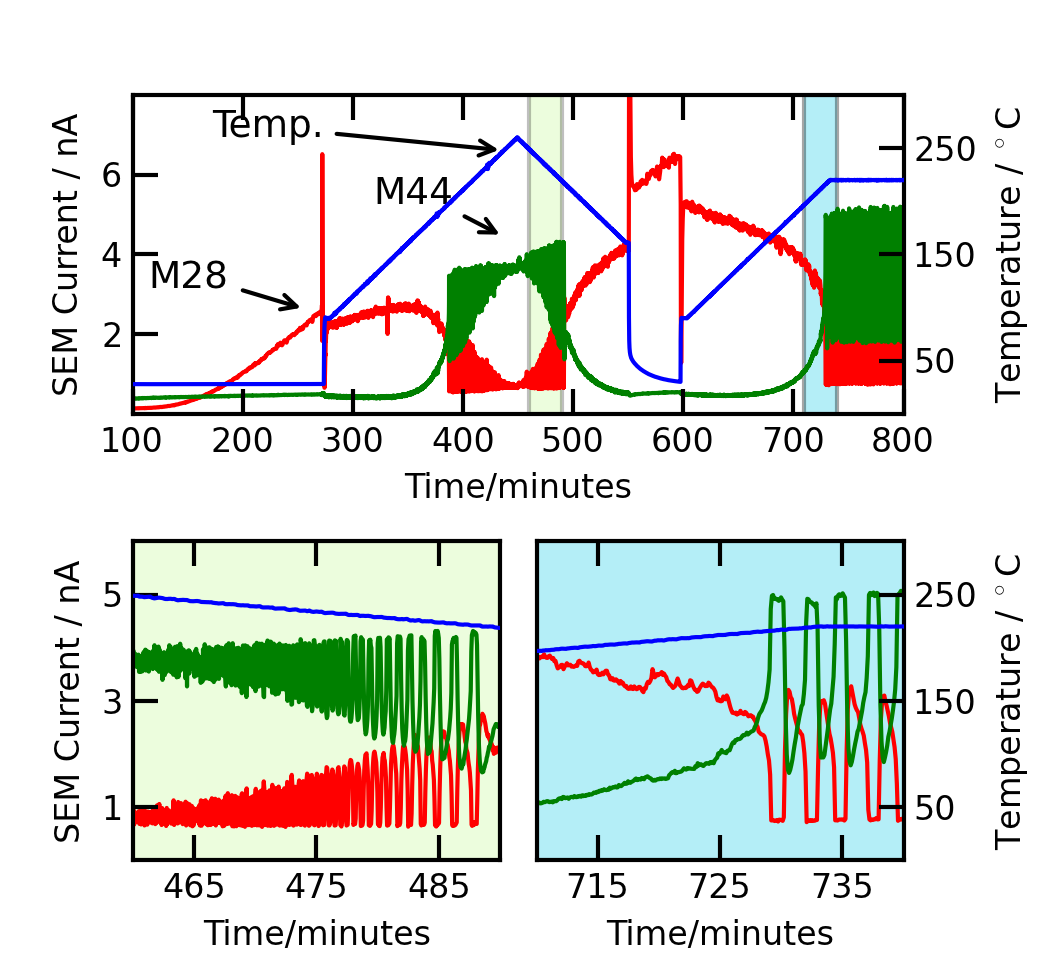
\includegraphics[width=12cm]{initial_treatment.png} 
  \caption{A typical example of the initial treatment of a new sample. After
  performing a light-off ramp, where oscillations can been seen, the temperature
  is increased to a constant value where sustained oscillations take place. The
  non-zero value of CO during high conversion periods is consistent with the
  expected QMS background signals from CO$_2$ and O$_2$.}
  \label{fgr:initial_treatment}
\end{figure}

The oscillations on all samples are qualitatively similar but the oscillation
period varies from a few seconds (the time constant of the reactor is
$\sim7\,$s) up to more than an hour. Once a sample starts to oscillate it will
perform self-sustained oscillations for as long as the experiment is allowed to
run. We have not observed a single sample stop oscillating once the self-sustained oscillations had started.

An example of a single very slow oscillation is seen in
Figure~\ref{fgr:full_oscillation}. After a short on-cycle (at $\sim$1030\,min) where
all CO is converted to CO$_2$ the reaction shows a fast deactivation. 
Notice the CO signal does not go to zero due to the cracking pattern of
CO$_2$ and CO background in the Quadrupole Mass Spectrometer (QMS).
After the deactivation the sample quickly regains
$\sim$30\% conversion (at $\sim$1040\,min). Hereafter the conversion increases
slowly over time until approximately 50\% conversion is reached (at
$\sim$1118\,min). Shortly after reaching 50\% conversion the sample again
ignites and converts all CO to CO$_2$. After a short full conversion period the
sample again deactivates and the cycle repeats itself.

Due to the long timescales between full conversion and low conversion plateaus
the oscillations cannot be attributed to the reactor setup itself which due to
its small size has timescales on the order of seconds. Furthermore, a series of
experiments were performed to exclude the oscillations as an instrumental
artifact. Firstly, experiments were performed on a reactor with five times larger volume and thus
five times increased residence time in the reactor. Secondly, the oscillations were
reproduced on a comparable but not identical setup. Finally, attempts at
reproducing the phenomenon on Pt thin films of comparable coverage did not
produce any oscillations. All of these experiments suggest that the
oscillations is a property of the Pt nanoparticles. However, 
although oscillations have previously been observed on extended Pt thin films
\cite{Singh2010} as well as single crystals\cite{Hendriksen2005} at atmospheric
pressure no oscillations could be provoked on thin films of comparable
geometrical coverage to the nanoparticles in our system at any CO/O$_2$ ratio.

\begin{figure}
  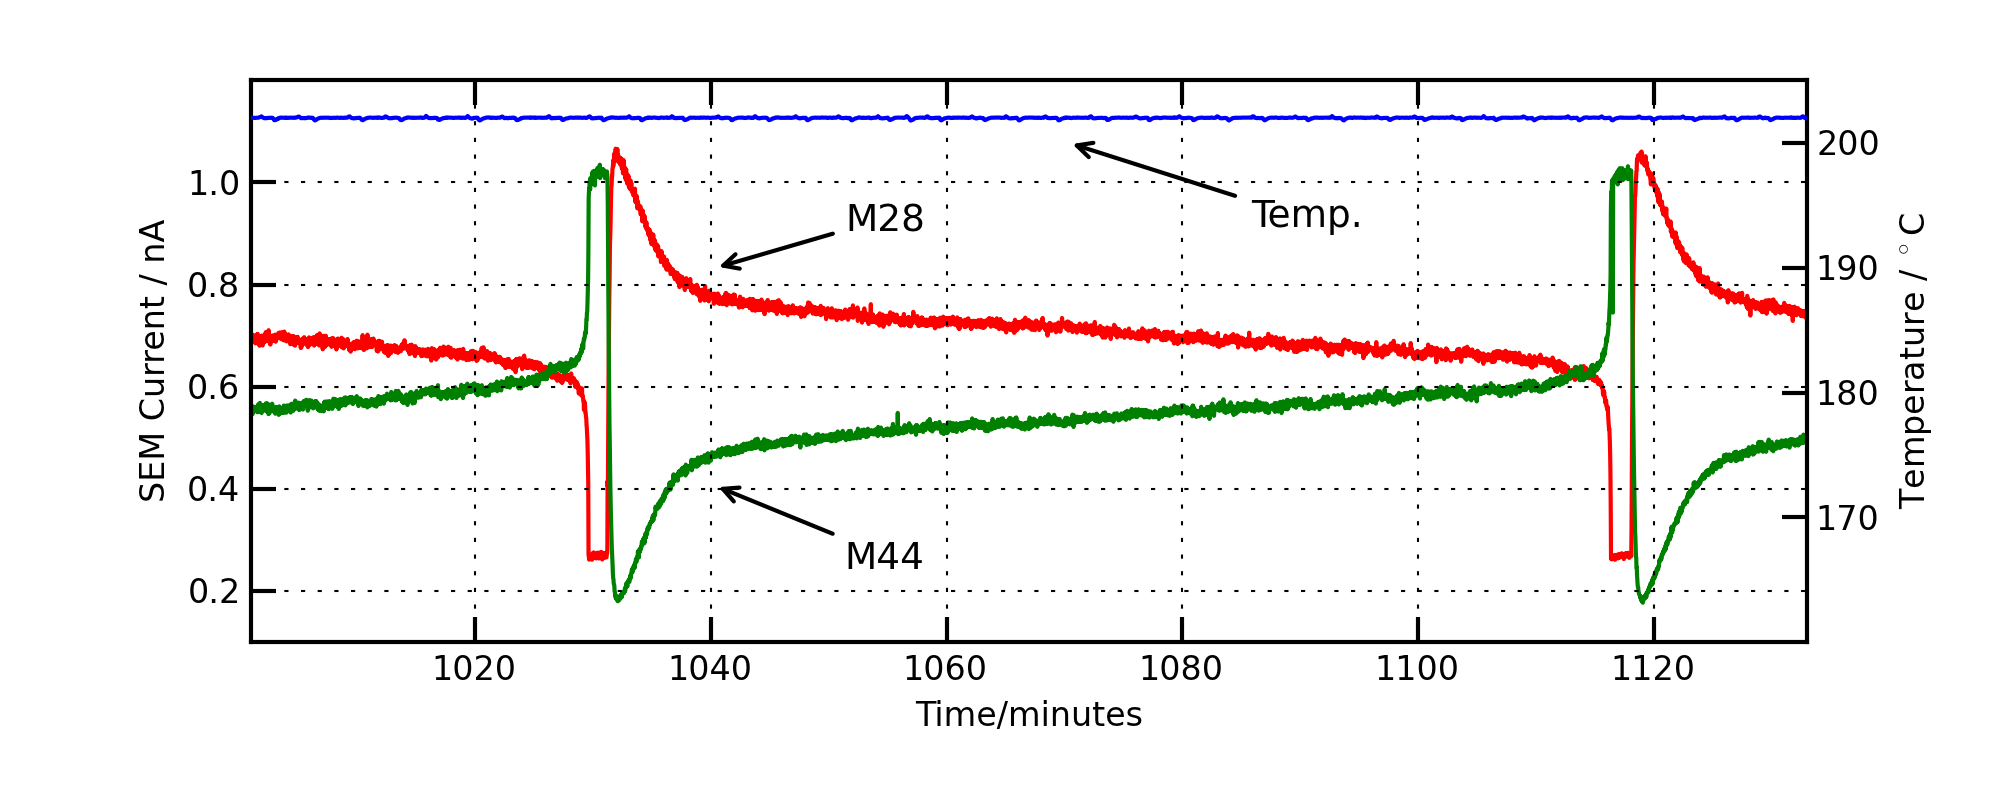
\includegraphics[width=16cm]{single_full_oscillation.png}
  \caption{A full oscillation period first showing a steep ignition of the
  sample followed by an almost immediate deactivation. For the next 65 minutes
  the sample slowly recovers activity until full conversion is reached again
  and the cycle repeats itself. This extremely long oscillation period is not
  commonly seen and was a result of careful parameter tuning. Typical
  oscillation periods are normally between $\sim$30\,s and $\sim$30\,min.
  Inserted circles illustrates the proposed model. At high conversion the
  platinum is oxidized (red) while in low conversion the sample is reduced
  (blue).} \label{fgr:full_oscillation}
\end{figure}

After prolonged measurements over several days an increase in oscillation
period was observed as shown in Figure~\ref{fgr:long_measurement}. Initially, the
oscillation period is $\sim$2.5 min and it increases linearly with time until 1500\,min
of total oscillation time. Hereafter the oscillations become more irregular
as shown in Figure~\ref{fgr:long_measurement} and in the lower panel of Figure~\ref{fgr:extracts}. At
experiment end the oscillation period is between 20\,min and 45\,min.

\begin{figure}
  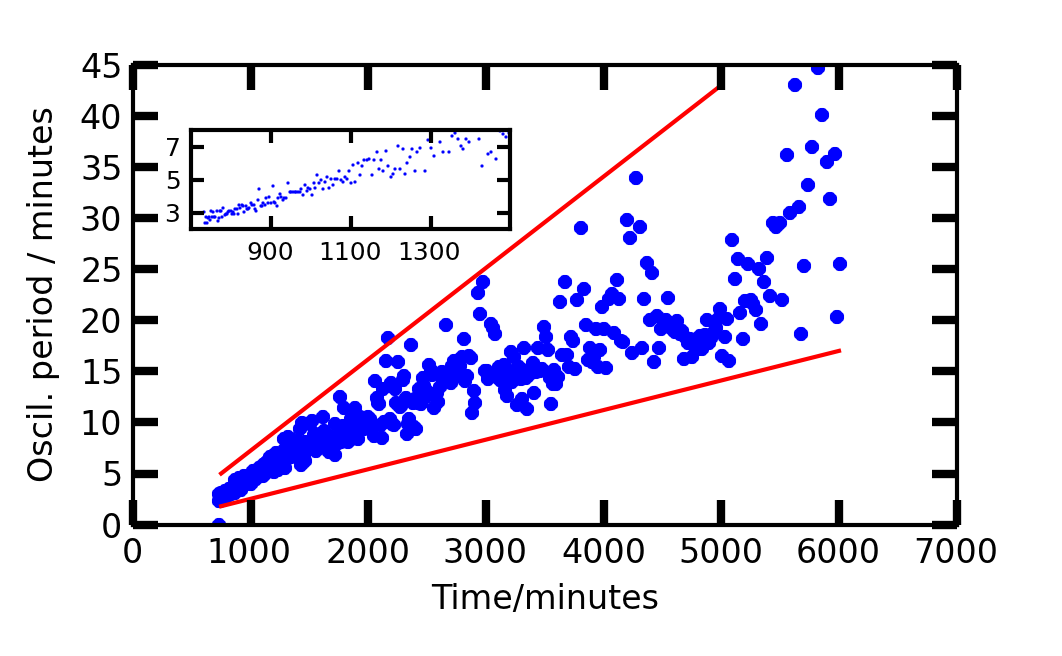
\includegraphics[width=12cm]{summary_of_long_measurement.png}
  \caption{Summary of the oscillation period as a function of time for a sample
  oscillating under constant temperature, pressure and reactant composition.
  The sample went through a total of 439 oscillations in 4 days. For details on on
  the oscillations over this period please consult supplementary Figure ????. Time is
  defined from experiment start and hence includes initial treatment. The inset
  shows the initial steady increase in oscillation period. The red lines indicate
  max and min oscillation time to guide the eye.}
  \label{fgr:long_measurement}
\end{figure}
  
Figure~\ref{fgr:extracts} shows extracts of mass spectrometry data of oscillations
extracted from the same four days measurement. Data from shortly after the
initial treatment, after 2800\,min of oscillation time and after 5900\,min are
shown. After 5900\,min the oscillations are more irregular which is consistent
with the data shown in Figure~\ref{fgr:long_measurement}. Also, oscillations in
between full conversion oscillations with smaller amplitude and much higher
frequency than the full on-off cycles become more visible as time progresses.
\begin{figure}
  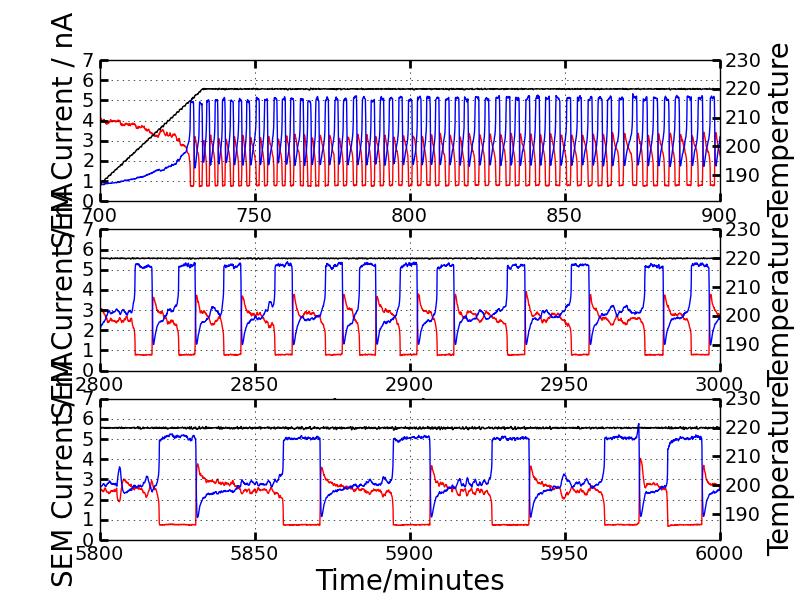
\includegraphics[width=12cm]{extracts_from_very_long_oscillation.png}
  \caption{Extracts from a 4 days long experiment. The oscillation period
  becomes more irregular with time while the total integrated conversion
  remains constant. Furthermore, small oscillations in between full conversion
  cycles become more prominent as time progresses.} \label{fgr:extracts}
\end{figure}

The oscillation period increases with time and becomes increasingly less stable
as shown in Figure~\ref{fgr:extracts}. This phenomenon is consistent across all
measured samples. The large scatter in oscillation period can be attributed to
the smaller oscillations in between on/off cycles. Occasionally, these small
amplitude oscillations will trigger a full switch thus introducing more
short-period oscillations despite the trend of increasingly longer oscillation
period. A possible explanation of the phenomenon could be sintering of the
particles during the oxidation and reductions cycles. However, the ratio
between CO and CO$_2$ integrated over an full period remains constant
throughout the entire experiment time, i.e. the samples maintain a constant
average rate independent of oscillation frequency. Thus we do not expect
sintering to be the cause since an average loss in activity of the sample would
be expected.

It has previously been shown using STM \cite{Hendriksen2002}, FT-IR
\cite{Carlsson2006}, Monte Carlo simulations \cite{Zhdanov2002} as well as DFT
\cite{Gong2004} that the activity of Pt towards CO oxidation at atmospheric
pressures is highly dependent on the oxidation state of the surface. A detailed
proposal for the reaction mechanism on Pd has been developed by Hendriksen
\textit{et. al.}\cite{Hendriksen2010} and our data are consistent with this
model.

According to the proposed model in ref.~\citenum{Hendriksen2010} the bare metal
surface is less active than the oxidized surface. Oscillations originate from a
switch between an oxidized surface and the bare metal surface. Initially, with
CO present in the inlet gas a smooth metal surface is exposed due to the
general high adsorption energy of CO on metal surfaces. As the Pt nanoparticles
convert the CO to CO$_2$ the partial pressure of CO will decrease and a Pt
oxide will start to form in the high partial pressure of O$_2$ thus increasing
the rate. The model\cite{Hendriksen2010} suggests that the oxidized
nanoparticles will roughen during CO oxidation resulting in the formation of an
increasingly rough oxide surface. As the oxide becomes rougher the bare metal
surface is increasingly favored resulting in a return to the lower rate rough
metal state. As the rate decreases the CO partial pressure increases which
results in a transition from rough metal surface to a smooth metal surface.
When the sample is sufficiently smooth it will again oxidize and thus complete
the oscillation cycle.

\subsection{Temperature dependence}
\begin{figure}
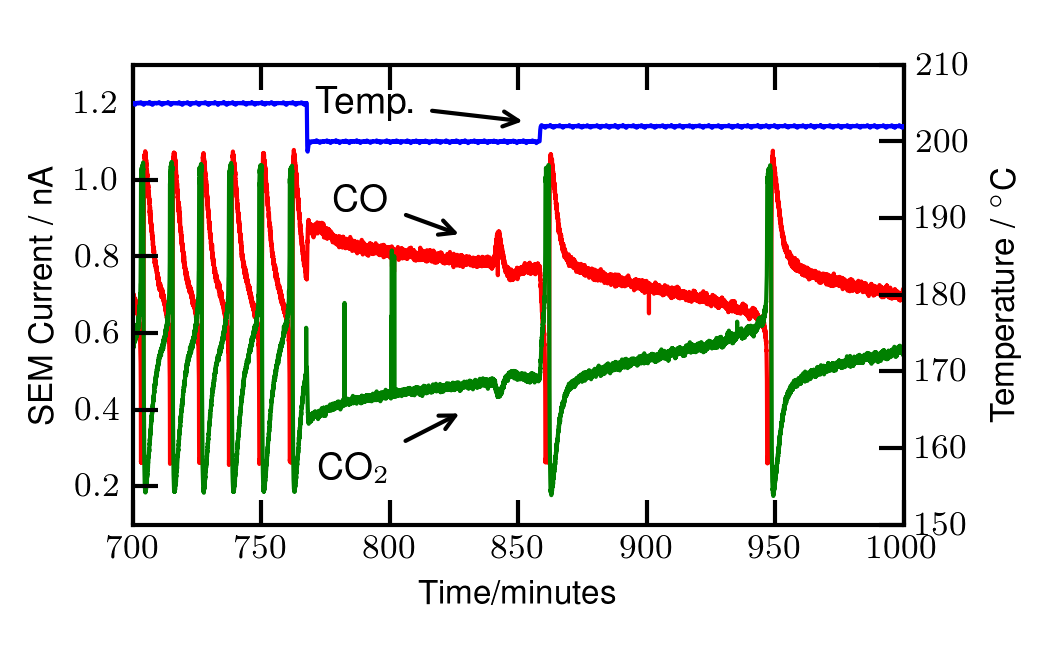
\includegraphics[width=12cm]{temperature_dependence.png}
\caption{Illustration of the strong temperature dependence of the oscillation period. After about 10
  hours of steady oscillations at 205\,$^\circ$C the temperature is lowered by
  5\,$^\circ$C immediately decreasing the oscillation frequency. The temperature
  is hereafter increased by 2\,$^\circ$C resulting in an increase in oscillation
  frequency. At 205\,$^\circ$C the oscillation period was approximately 500\,s
  while the oscillation period period is approximately 5000\,s. at
  203\,$^\circ$C.
  \label{fgr:temperature_dependence}
}
\end{figure}

An interesting feature in the data is the very large temperature dependence of the
oscillation frequency as shown in Figure~\ref{fgr:temperature_dependence}. By
changing the temperature 5\,$^\circ$C the oscillation period was changed by more
than a factor of 10. The magnitude of the change is not completely consistent
across all measured samples but all samples show a very large temperature
dependence. In some cases a provoked change in temperature will
consistently turn on and off the oscillations. This is illustrated in the supplementary
material, Figure ??????\ref{fgr:temperature_dependence_supplemental}.
\begin{figure}
\centering
  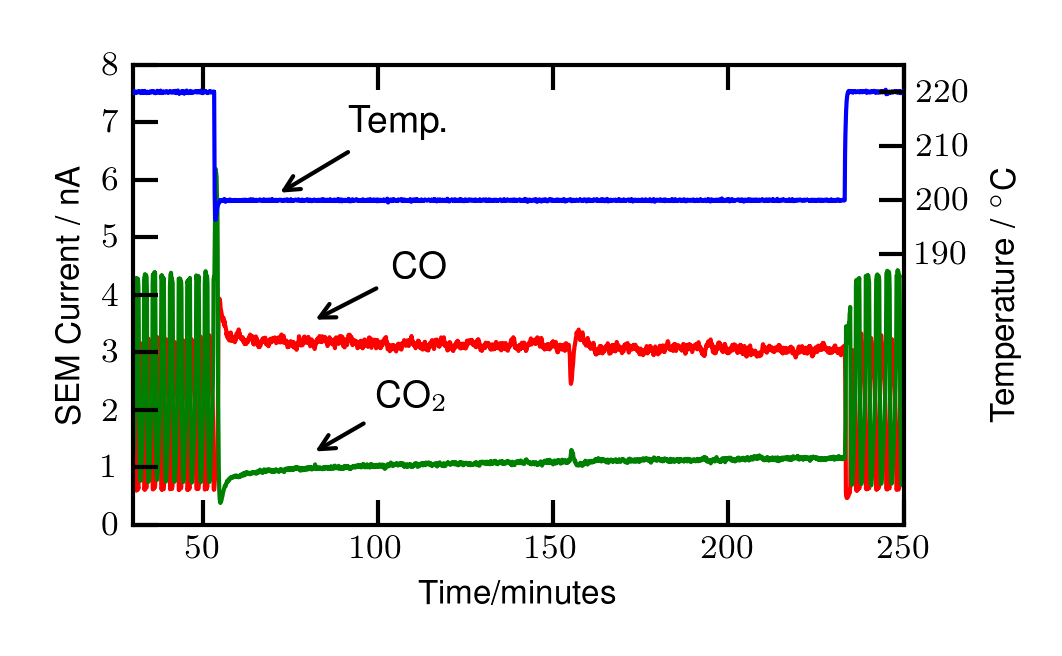
\includegraphics[width=12cm]{temperature_dependence_supplemental.png}
  \caption{Another example of the very pronounced temperature dependence of the oscillation period.
  Here the oscillations are turned on and off by changing the temperature by
  $20^\circ$C.}
  \label{fgr:temperature_dependence_supplemental}
\end{figure}
This property agrees well an earlier suggested model \cite{Hendriksen2010} and
it is, to our knowledge, the first time the temperature dependence of
oscillations at atmospheric pressure has been measured.

\subsection{Pressure dependence}
The pressure dependence of the oscillations was also investigated. In the
pressure range of 0.1\,bar to 1\,bar no change of the oscillation frequency or
qualitative behavior that could be attributed to the pressure was found.
Similarly, only a weak dependence on the CO/O$_2$ ratio was observed. At a
CO/O$_2$ ratio of $\sim0.025$ only very small amplitude oscillations were
observed. Increasing the CO/O$_2$ ratio showed clear oscillations with a significant
increase in oscillation amplitude compared to lower CO concentrations.
Generally, a tendency towards longer oscillation periods for higher CO/O$_2$
ratio was observed. Richer CO mixtures than 0.175 did not produce any
oscillations in our system.

%No consistent dependency on oscillation frequency and duty cycle was found that could be attributed to the size of the particles.

\subsection{CO concentration dependence}
The dependence of period of the oscillations on the the CO concentration was
investigated. The result shows that the period increases slightly with
increasing CO-concentration. However, the effect is small compared to the
general trend of slower oscillations as the experiment progresses. In
Figure~\ref{fgr:gas_dependence_summary} the oscillation periods are summarized and the
actual mass spectrometry data of the entire experiment are shown in Figure~\ref{fgr:gas_dependence}.

\begin{figure}
  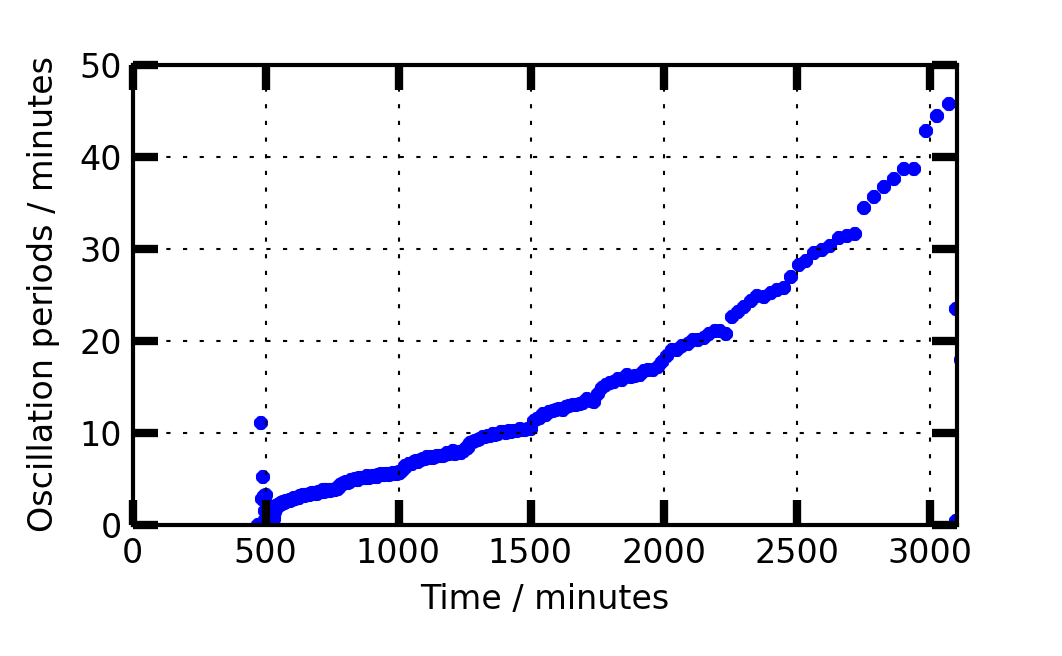
\includegraphics[width=12cm]{oscillations_gas_dependence_summary_supplemental.png}
  \caption{Oscillation period (blue) as a function of time and CO concentration (black). The
  overall trend of increasing oscillation period with time is superimposed with small
  discontinuous steps when the CO concentration is increased.} 
  \label{fgr:gas_dependence_summary}
\end{figure}

Oscillations were only seen in CO/O$_2$ ratio below 0.175. This ratio agrees
well with literature \cite{Singh2010,Hendriksen2005} where oscillations have
been observed in oxygen rich CO/O$_2$ mixtures. The needed low concentration of
CO in the inlet gases can be attributed to the much higher sticking coefficient
of CO on Pt which poisons the nanoparticle surface during the low reactivity
region of the cycle.

\begin{figure}
  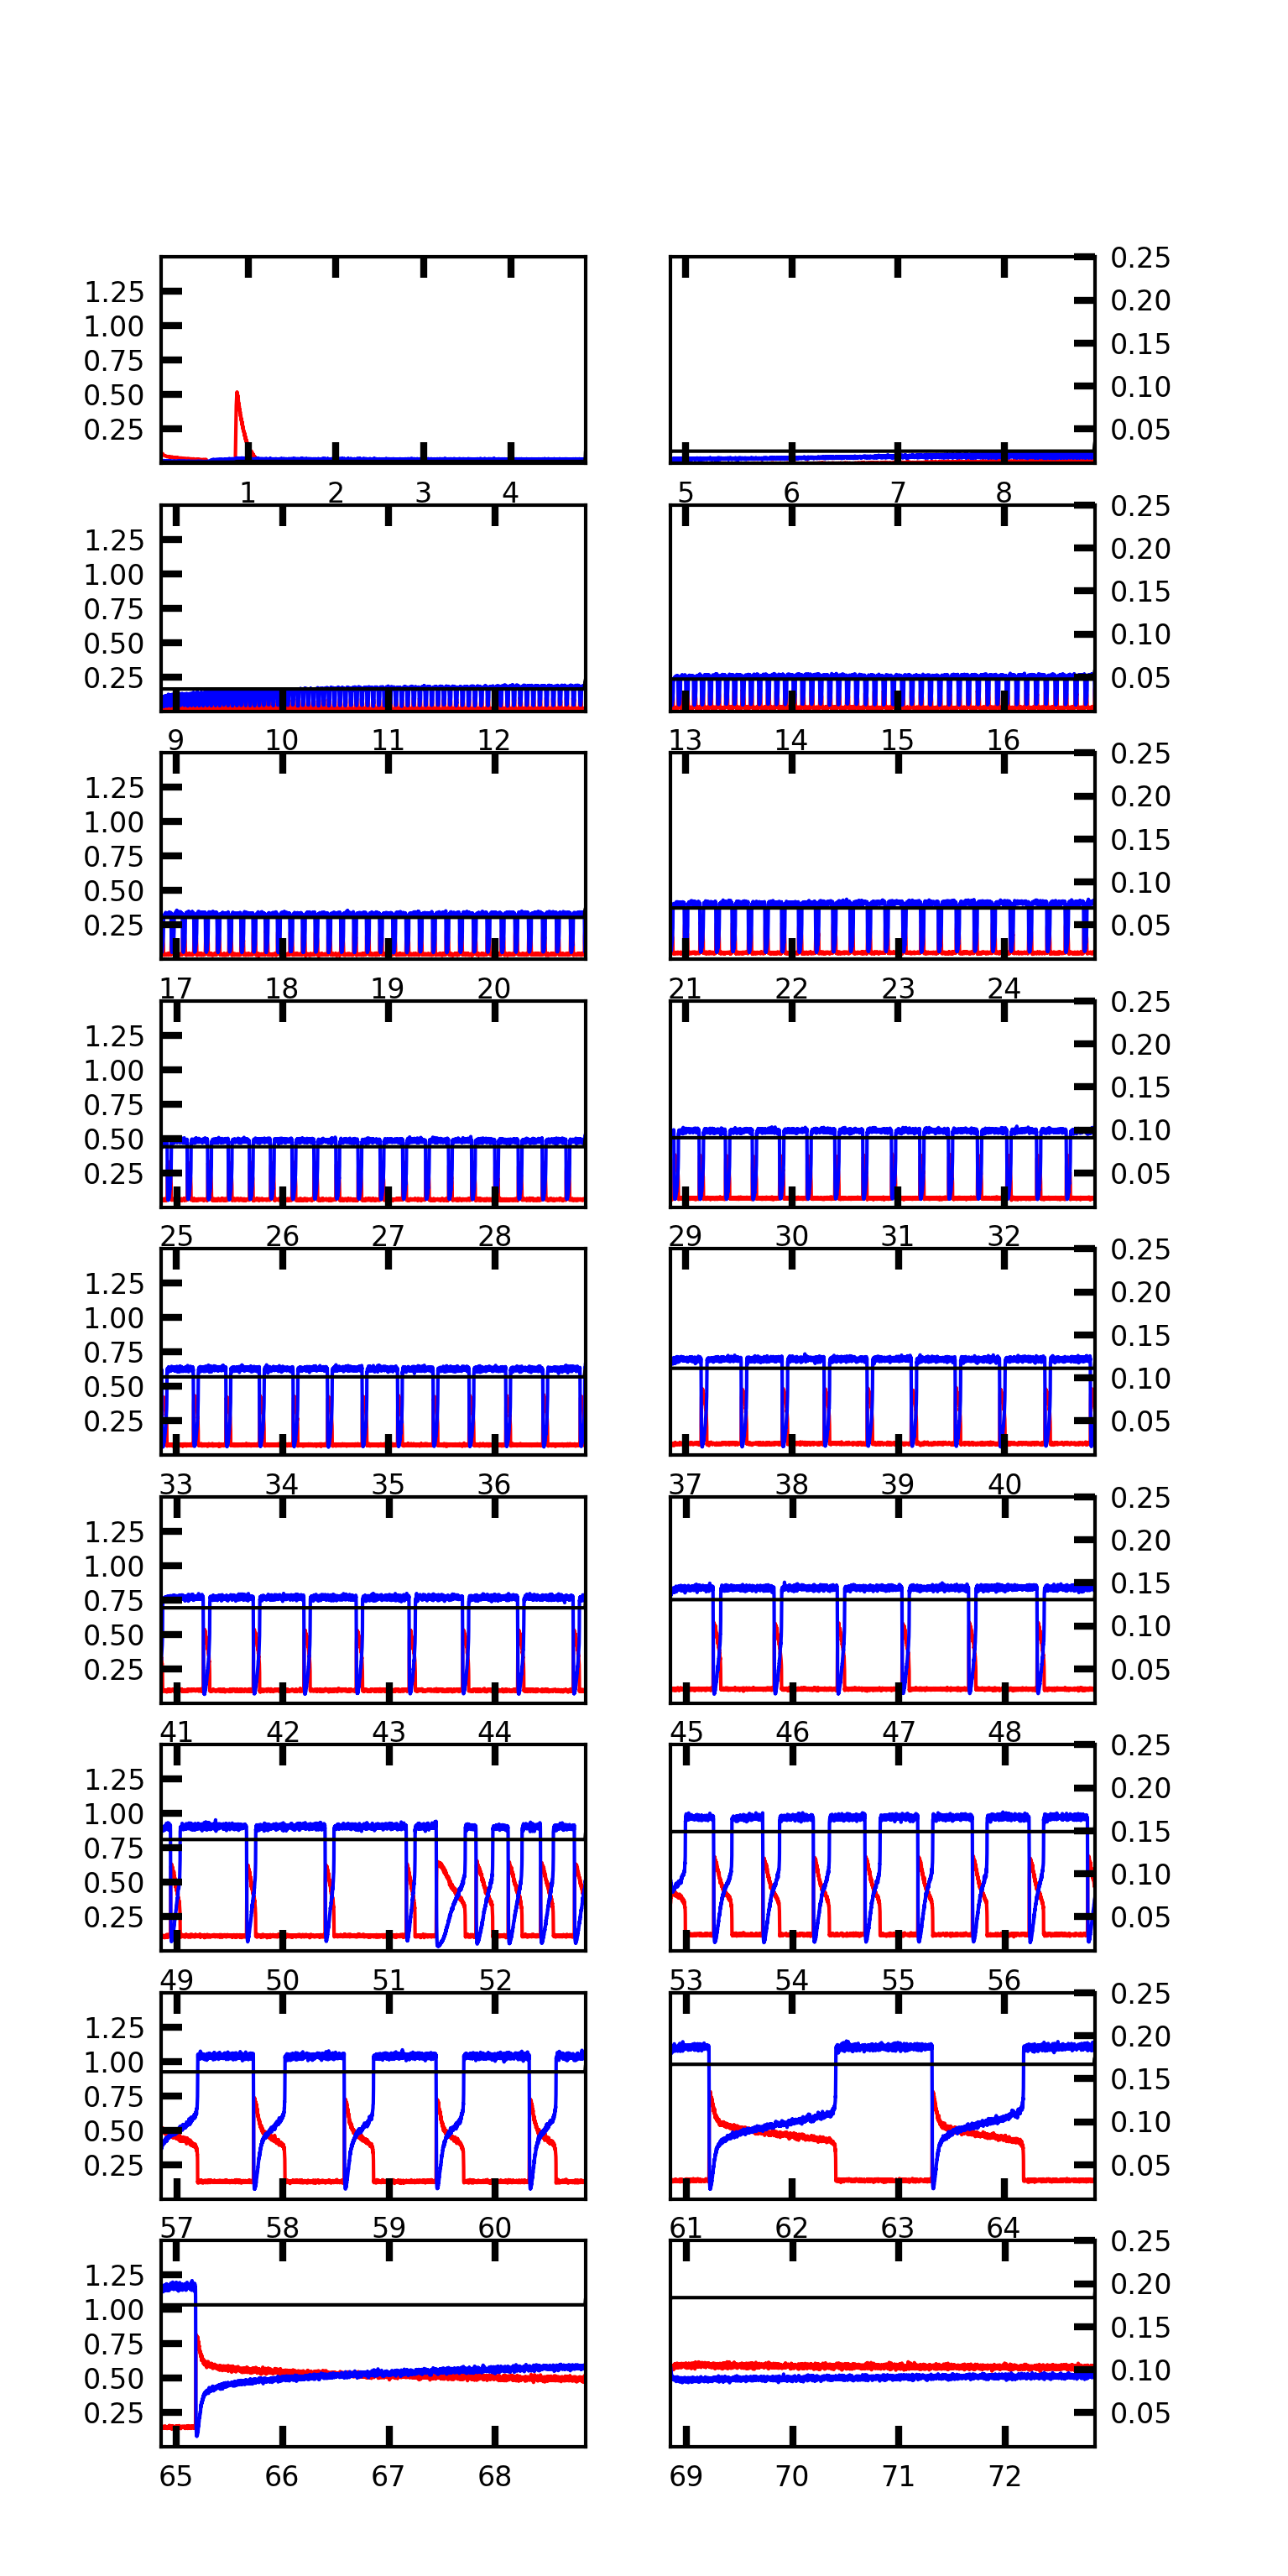
\includegraphics[width=14cm]{oscillations_gas_dependence_supplemental.png}
  \caption{Complete series of data from an oscillating sample, showing CO (red) and CO$_2$
  (blue). The temperature is constant at $210^\circ$C during the entire
  measurement. For every frame the CO-concentration is increased.}
  \label{fgr:gas_dependence}
\end{figure}

\subsection{Duty cycle}
Even though the period of the oscillations increases with time the total
integrated conversion rate during a complete cycle is almost constant. In
Figure~\ref{fgr:duty_cycles_supplemental} the mean value of CO and
CO$_2$ is plotted for every oscillation in a four-day long experiment. It is
evident that the ratio between CO and CO$_2$ is almost constant. The
average activity of the sample is thus almost unchanged despite the development in
the oscillation frequency.

\begin{figure}
  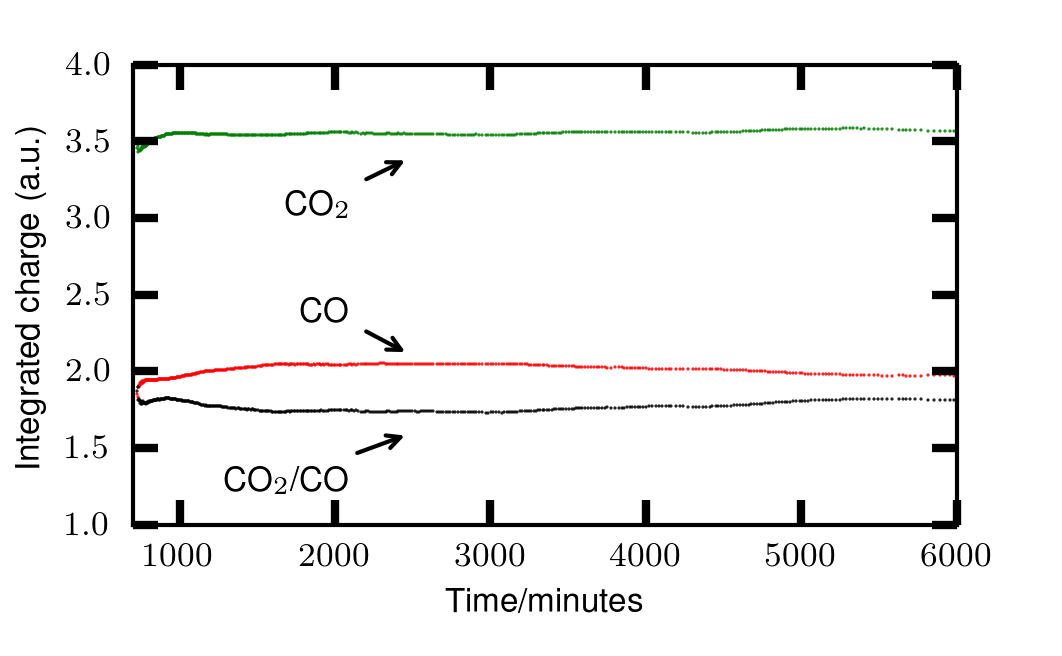
\includegraphics[width=12cm]{duty_cycles_long_measurement_supplemental.png}
  \caption{Running average of the CO and CO$_2$ concentrations and their ratio during a 4-day long
  experiment. The individual data-points is calculated as the integral of CO
  (red) or CO$_2$ (green) during the individual oscillation periods. The ratio between
  CO and CO$_2$ is drawn in black.} \label{fgr:duty_cycles_supplemental}
\end{figure}

\subsection{Size dependence}
Nanoparticles with sizes ranging from 3\,nm to 9\,nm have been tested but 3\,nm
particles with a geometrical coverage of 0.1\% of the reactor area gave the
most stable oscillations. 
However, no change in duty cycle or frequency that could be
attributed to the size of the nanoparticles was found. This may be due to the
fact that even nominally identical samples also show a large variation in
oscillation frequency and duty cycle thus possibly shadowing a nanoparticle
size effect.


\subsection{Proposed mechanism}
In this study Pt nanoparticles were investigated which, compared to a single
crystal or a thin film, have a very rough surface. It is to be expected that the
particles will initially favor the reduced state. As the reaction runs the gas
composition towards the outlet of the reactor will become more oxidizing
increasing the oxidation rate of the particles (illustrated in the bottom of
Figure~\ref{fgr:full_oscillation}). Gradually, as the particles towards the outlet
oxidizes the turn-over frequency will increase and the general CO concentration will
decrease promoting more and more particles to oxidize which will gradually be
seen in the QMS as an increase in CO$_2$ and a decrease in CO. As the CO
concentration decreases the light-off temperature will decrease hence
approaching the constant temperature of the sample resulting in a steep
increase in reactivity. It is important to note that the fraction of oxidized
particles needed to achieve full conversion is not known. We are currently
investigating new methods for gaining insight into the nature of the
nanoparticles in the reactor but the low coverage and the design of the reactor
makes this a challenging task. If all particles are not oxidized at light-off
they will now oxidize much faster due to the low CO-concentration. The further
increased rate will not be visible in the QMS since the reactor is already in
full conversion. As most of the particles are now oxidized they will become
more and more roughened and gradually return to the reduced state. Fewer and
fewer oxidized particles will be responsible for the activity increasing the
roughing rate of the remaining active particles. Just before the overall
activity drops only a fraction of the particles participates in the reaction
and the deactivation will happen very suddenly. Once these potentially few
particles eventually becomes sufficiently rough they will reduce and lose
activity hence completing the oscillation cycle. It should be noted that our
group has recently measured turnover frequencies of CO oxidation on Pt in
excess of $10^{6}$\,s$^{-1}$ per site corresponding to as little as $\sim$300 Pt
nanoparticles contributing to the reactivity just before the end of the high-
activity cycle. This would correspond to an area of ????? ppm of the reactor
area suggesting that in situ studies are becoming a challenges as such a
minority of the reactor volume could account for all the reactivity. Attempts
to see any thermal signal from such small areas has so far been in vain.

\section{Conclusions}
Self-sustained CO oxidation oscillations at atmospheric pressure on Pt
nanoparticles ranging from from 3\,nm to 9\,nm in diameter have been measured with
high-quality mass-spectrometry. Full conversion was achieved on 0.1\,\%
geometrical Pt coverage and it is found likely that full conversion can be obtained on
extremely small amounts of Pt. It was found that the samples increased the
oscillation period over time and showed a strong temperature dependence of the
oscillation period. A model is proposed where the nanoparticles go through repetitive
oxidation/reduction cycles which change the change rate of CO oxidation on the
particles. The fact that extremely few NP may account for the activity make in
situ investigations a challenge.


\section{Experimental Methods}
\subsection{The $\mu$-reactor platform}
The experiments were performed in Si-based 20x16\,mm
$\mu$-reactors\cite{Henriksen2009}. The reactor consists of two inlets, a
mixing zone allowing for diffusional mixing of reactants, an outlet, a reactor
volume of $240\,$nL and a $5.4\,\mu$m wide, 3\,$\mu$m high and 1500\,$\mu$m
long capillary used for sniffing gases from the reactor volume. The reactor is
sealed by anodic bonding of a Pyrex lid to the Si reactor and is able to
operate in a pressure range of 0--2.5\,bar. The reaction gases are supplied to
the two inlets by flow controllers capable of controlling the gas flow from 0--
10 mL/min. The capillary flow is fed into a QMS
for analysis while any surplus of gas from the inlets is passed directly
through to the outlet via a pressure controller allowing control of reactor
pressure. The design makes sure that all gases exposed to the catalyst under
investigation are measured by the QMS ensuring an extremely high sensitivity of
the system. 

\begin{figure}
 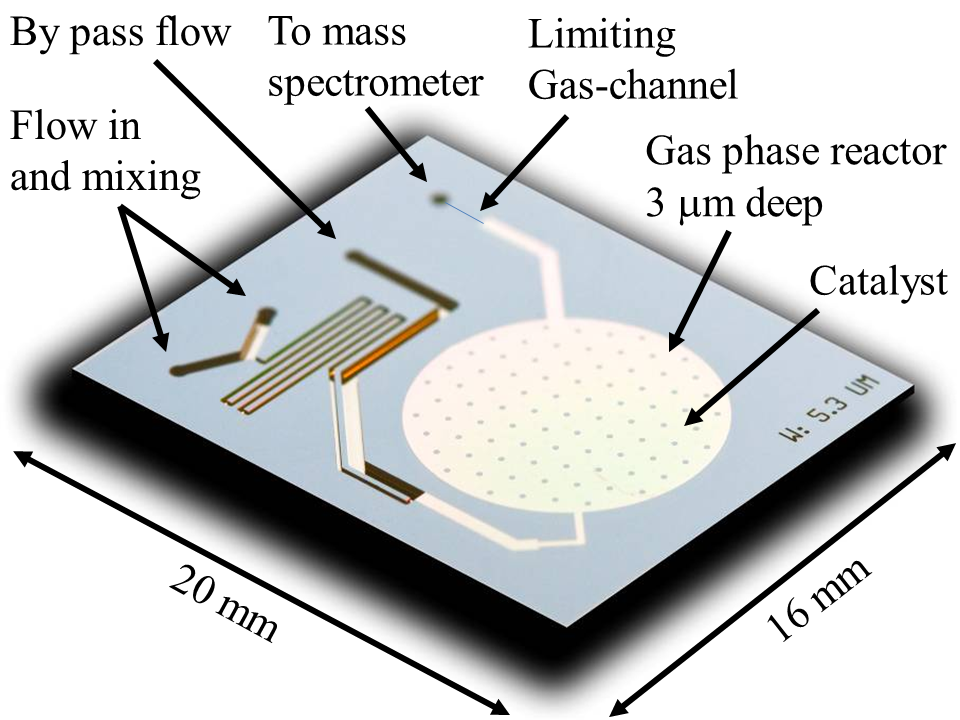
\includegraphics[width=8cm]{Ib-reactor.png}
 \caption{Image of the 20x16\,mm microreactor showing the circular reactor area
and the gas channel system.}
  \label{fgr:reactor}
\end{figure}

Before any measurements are performed the reactor is evacuated by a turbopump to minimize
contaminants in the system. When an evacuated reactor is mounted the base
pressure of the mass spectrometer chamber is $\sim5\times10^{-9}\,$mbar and in
operation at $1\,$bar in the reactor volume the pressure is
$\sim5\times10^{-7}\,$mbar in the QMS chamber.

The reactor is heated by joule heating of a Pt strip evaporated on the backside
of the reactor chip. The introduction of two additional contacts on the
backside of the reactor allows for 4 wire measurements of the resistance of the
Pt strip using it as a RTD for temperature measurement of the reactor. An
external thermocouple acts as room-temperature calibration of the RTD as well
as a sanity check of the RTD measurement during operation. The measured RTD
temperature is always compared to the thermocouple temperature at room temperature both
before and after an experiment to be sure the RTD did not change resistance due
to annealing during the experiment.

The gas handling including flow and pressure controllers and the mass
spectrometer is fully automated allowing for measurements during several days
without human intervention allowing for self-consistent measurements of many
samples.

\subsection{Pt nanoparticle deposition}
Pt nanoparticles were deposited in the reactor using a gas-aggregation source
(Mantis Deposition Ltd., Nanogen 50). Pt clusters were formed by gas-phase
condensation of Pt atoms produced by impinging argon ions on a 99.99\% Pt
target in a magnetron sputter source. After condensation the ionised fraction
(60-80\%) of the clusters is size-selected by a quadropole mass selection
filter according to their mass-to-charge ratio. Using this setup Pt
nanoparticles with diameters in the range of 2--16\,nm can be produced
\cite{Nielsen2010,Nielsen2009}. The size-selected nanoparticles were after
size-selection soft-landed in the reactor volume of the microreactor. The
coverage was kept at approximately 0.1\% geometric coverage determined by
measuring the current on the reactor during deposition. After deposition the
reactors were anodically cold-bonded \cite{Vesborg2010} to a pyrex lid to avoid
sintering of the nanoparticles while bonding in air.

\section{Acknowledgments}
This work was carried out as part of the Catalysis for Sustainable Energy
initiative, which is funded by the Danish Ministry of Science, Technology and
Innovation. The Center for Individual Nanoparticle Functionality is funded by
the Danish National Research Foundation.


\bibliography{literature} %your .bib file


\end{document}
